% SPDX-FileCopyrightText: 2026 Alexander S. Donahue
% SPDX-License-Identifier: CC-BY-4.0
\documentclass[11pt,reqno]{amsart}

\usepackage[margin=1in]{geometry}
\usepackage[T1]{fontenc}
\usepackage{lmodern}
\usepackage{microtype}
\usepackage{amsmath,amssymb,amsthm,mathtools}
\usepackage{booktabs,array,tabularx}
\usepackage{graphicx}
\usepackage{xcolor}
\usepackage{xurl}
\usepackage[colorlinks=true,linkcolor=blue!65!black,citecolor=teal!70!black,urlcolor=blue!65!black]{hyperref}
\usepackage[nameinlink,noabbrev]{cleveref}

\newtheorem{theorem}{Theorem}[section]
\newtheorem{proposition}[theorem]{Proposition}
\newtheorem{lemma}[theorem]{Lemma}
\newtheorem{corollary}[theorem]{Corollary}
\theoremstyle{definition}
\newtheorem{definition}[theorem]{Definition}
\newtheorem{remark}[theorem]{Remark}
\newtheorem{conjecture}[theorem]{Conjecture}

\newcommand{\R}{\mathbb{R}}
\newcommand{\C}{\mathbb{C}}
\newcommand{\N}{\mathbb{N}}
\newcommand{\Z}{\mathbb{Z}}
\newcommand{\Q}{\mathbb{Q}}
\newcommand{\sinc}{\operatorname{sinc}}
\newcommand{\Var}{\operatorname{Var}}
\newcommand{\taglean}{\textsc{[lean-6k]}}
\newcommand{\tagexact}{\textsc{[exact-comp]}}
\newcommand{\tagnum}{\textsc{[num-approx]}}
\newcommand{\tagemp}{\textsc{[empirical]}}
\newcommand{\id}[1]{\textnormal{\texttt{\small #1}}}
\newcommand{\idb}[1]{\textnormal{\texttt{\footnotesize #1}}}
\newcommand{\ub}{\_\allowbreak}

\title[The Spectral Eclipse Frontier]{The Spectral Eclipse Frontier: Complete Resolution of Conjecture~4.1, Sharp Even/Odd Rupture Thresholds, Universal $3R+2$ Phase Transition, Non-Symmetric Complex Eclipses, and Quantum Geometric Speed Limits}

\author{Alexander S. Donahue}
\address{Independent Researcher, Spokane, WA, USA}
\email{0\_0@0thernes.art}
\urladdr{https://orcid.org/0009-0006-8168-9648}

\date{November 27, 2026 (Version 1.1.0 --- Unrefereed Research Preprint)}

\keywords{Perfect state transfer, early state exclusion, persymmetric Jacobi matrices, Hochstadt inverse spectral theorem, divided differences, Bernstein polynomials, Mandelstam--Tamm quantum speed limit, Fubini--Study metric, Lean 4 formal verification}
\subjclass[2020]{81P45, 15A29, 33C45, 42A05, 68V20}

\begin{document}

\begin{abstract}
A one-dimensional $XX$ spin chain with persymmetric Jacobi Hamiltonian $J$ exhibits \emph{Perfect State Transfer} (PST) at time $T_0$ when $|\langle e_{N-1}, e^{-i J T_0} e_0\rangle|=1$, and \emph{Early State Exclusion} (ESE) when the return amplitude $A(t)=\langle e_0, e^{-i J t} e_0\rangle$ vanishes strictly before transfer, i.e., at some $\tau\in(0,T_0)$. Recently, Escobar, Garcia, and Minenkova (\texttt{arXiv:2507.18767v1}) conjectured (Conjecture~4.1) that a symmetric $7\times 7$ PST spin chain with spectrum $\{0,\pm\lambda_1,\pm\lambda_2,\pm\lambda_3\}$ avoids ESE if and only if $\lambda_1\mid\lambda_2$ and $\lambda_1\mid\lambda_3$, and raised the broader question of how divisibility governs ESE across higher dimensions and non-symmetric chains.

We resolve Conjecture~4.1 completely and establish a unified ten-theorem architecture governing ESE across arbitrary chain lengths, spectral symmetries, and quantum geometry:
\begin{enumerate}
\item \textbf{Complete low-dimensional dichotomies (Theorems~1--4):} We prove exact necessary and sufficient divisibility dichotomies for symmetric PST chains of lengths $N\in\{4,5,6,7\}$, resolving Conjecture~4.1 in both reduced and arbitrary real-scaled unreduced forms via a strictly decreasing secant-slope principle for $H(w)=\sinc^2(\sqrt{w})$ and a discrete Fourier coset-averaging theorem.
\item \textbf{Sharp even and odd rupture dimensions (Theorems~5--7):} We prove that minimal-gap divisibility \emph{ruptures} sharply at $N_{\mathrm{crit}}^{\mathrm{even}}=8$ (for all $m\ge 1$) and $N_{\mathrm{crit}}^{\mathrm{odd}}=11$ with exact integer cluster onset $M^*=12$ ($m\ge 6$, while all $m\in\{1,\dots,5\}$ are certified ESE-free by exact rational sum-of-squares certificates). Closing the gap between $7\times 7$ and $11\times 11$, we prove the \emph{Critical $9\times 9$ No-ESE Theorem}: \emph{every} $9\times 9$ symmetric PST chain $\{0,\pm 1,\pm b,\pm c,\pm d\}$ with alternating parity satisfies $A_9(t)>0$ on $[0,\pi)$, proved via a global second-divided-difference bound and $19$ exact bivariate Bernstein polynomial certificates.
\item \textbf{Universal $(R,r)$ phase transition (Theorem~8):} Fusing an equidistant $R$-eigenvalue Krawtchouk core with an $r$-pair unit-spaced spectral cluster ($N=R+2r$) produces a sharp three-regime asymptotic phase transition at $r_{\mathrm{crit}}(R)=R+1$, i.e., $N_{\mathrm{crit}}(R)=3R+2$, unifying $N=8$ ($R=2$) and $N=11, M^*=3\cdot 2^2=12$ ($R=3$).
\item \textbf{First infinite non-symmetric complex-amplitude ESE family (Theorem~9):} We construct explicit staggered-field $5\times 5$ persymmetric Jacobi matrices $J_{a,b}$ (diagonal $(b,b+2a,b,b+2a,b)$) for all odd $a$ with $3\nmid a$ and $b=a+6k+3$ achieving exact PST at $T_0=\pi$ and exact \emph{complex} ESE $A(\pi/3)=0\in\C$ despite unit minimal spectral gap.
\item \textbf{Quantum geometric speed limit and ESE--ETE duality (Theorem~10):} For every $N\times N$ Jacobi chain, the Quantum Geometric Tensor Fubini--Study metric at $|0\rangle$ equals $g_{tt}=b_0^2$, every ESE time obeys the Mandelstam--Tamm bound $\tau\ge\pi/(2|b_0|)$, and every persymmetric PST chain satisfies exact time-reversal duality $|\psi_{N-1}(T_0-t)|=|\psi_0(t)|$.
\end{enumerate}

All ten theorems (plus $18$ non-vacuity witnesses, $5$ adversarial refutations, and $12$ isolated Mathlib-only comparator targets) are formally machine-checked in Lean~4.35.0 ($572$ audited theorem constants; strictly standard axioms \texttt{[propext, Classical.choice, Quot.sound]}; zero \texttt{sorry}; zero Batteries linter errors) and independently cross-validated across eight polyglot and quantum engines with zero mismatches. Finally, we report a pre-registered $4$-arm QRNG static-disorder study ($K=30$ paired seeds), confirming significant eclipse persistence in real codimension-$1$ symmetric chains ($p_{\mathrm{Holm}}=0.0004$) and documenting an honest pre-registered null result for complex codimension-$2$ eclipses in $J_{1,4}$ ($p_{\mathrm{Holm}}=0.9855$).
\end{abstract}

\maketitle

\begin{center}
\fbox{\parbox{0.94\linewidth}{\footnotesize
\textbf{Epistemic Status \& AI-Assistance Disclosure.} This document is an \textbf{unrefereed research preprint} (v1.1.0; Master Archive ID \texttt{0TH-2026-024}) and has not undergone external peer review or journal submission. Analytical proof discovery, Lean~4.35.0 formalization, polyglot verification engineering, and manuscript drafting were conducted with AI assistance (Google Gemini / Antigravity) under the direction and audit oversight of the sole human author (Alexander S.~Donahue, ORCID \href{https://orcid.org/0009-0006-8168-9648}{0009-0006-8168-9648}). Every mathematical theorem tagged \taglean{} is verified end-to-end by the Lean~4.35.0 kernel without \texttt{sorry} or custom axioms and replayed across six independent checker runs via \texttt{lake comparator --paranoid}. Code and Lean proofs are licensed \texttt{Apache-2.0}; this manuscript and figures are licensed \texttt{CC-BY-4.0}. Repository: \url{https://github.com/0thernes/spectral-eclipse-frontier}.
}}
\end{center}

\tableofcontents

% ============================================================================
\section{Introduction and Summary of Verified Claims}
\label{sec:intro}

Quantum state transfer along nearest-neighbor spin-$1/2$ chains governed by an $XX$ Hamiltonian with site-dependent couplings $b_j>0$ and local magnetic fields $a_j\in\R$ reduces in the single-excitation subspace to unitary evolution $e^{-iJt}$ under an $N\times N$ real symmetric tridiagonal Jacobi matrix $J$~\cite{christandl2004,christandl2005,kay2010}. By the inverse spectral theory of Hochstadt~\cite{hochstadt1967,hochstadt1974} and the algebraic characterization of Christandl et al.~\cite{christandl2005}, Kay~\cite{kay2010}, Godsil~\cite{godsil2012}, and Vinet--Zhedanov~\cite{vinet2012}, Perfect State Transfer (PST) from site $|0\rangle$ to site $|N-1\rangle$ at time $T_0>0$ requires $J$ to be \emph{persymmetric} (mirror-symmetric about its anti-diagonal: $a_{N-1-j}=a_j$, $b_{N-2-j}=b_j$) and requires its distinct eigenvalues $\lambda_0<\lambda_1<\dots<\lambda_{N-1}$ to satisfy exact alternating-parity commensurability:
\begin{equation}
\label{eq:pst-cond}
\frac{(\lambda_k - \lambda_0)T_0}{\pi} \in 2\Z + (k \bmod 2) \qquad (k=0,1,\dots,N-1).
\end{equation}

While PST guarantees that the initial-site survival amplitude $A(t) = \langle e_0, e^{-iJt} e_0\rangle$ vanishes at the transfer instant $t=T_0$, Escobar, Garcia, and Minenkova~\cite{escobar2025} introduced the sharp dynamical phenomenon of \emph{Early State Exclusion} (ESE): the existence of a strictly earlier time $\tau\in(0,T_0)$ at which $A(\tau)=0$, meaning the excitation is completely absent from its launch site before arrival at the opposite end. Using exact spectral weights determined by Hochstadt's formula, they proved complete divisibility dichotomies for symmetric chains of lengths $N=4$ and $N=5$ and formulated:

\begin{conjecture}[Escobar--Garcia--Minenkova, {\cite[Conjecture~4.1]{escobar2025}}]
\label{conj:41}
Let $J$ be a $7\times 7$ symmetric persymmetric Jacobi matrix realizing PST at $T_0=\pi$ with spectrum $\{0,\pm\lambda_1,\pm\lambda_2,\pm\lambda_3\}$ ($0<\lambda_1<\lambda_2<\lambda_3$, alternating odd/even/odd integer ratios). Then $J$ has no Early State Exclusion on $(0,T_0)$ if and only if $\lambda_1\mid\lambda_2$ and $\lambda_1\mid\lambda_3$.
\end{conjecture}

This paper proves \Cref{conj:41} completely---and reveals that $N=7$ sits directly below a dramatic, previously unknown structural boundary. Contrary to the natural extrapolation that minimal-gap divisibility ($\lambda_1=1$) prevents ESE in all dimensions, we prove that divisibility \emph{survives} through $N=6$ (even) and $N=9$ (odd), and \emph{ruptures sharply} at $N_{\mathrm{crit}}^{\mathrm{even}}=8$ and $N_{\mathrm{crit}}^{\mathrm{odd}}=11$ (at exact onset $M^*=12$). Both ruptures are instances of a universal $(R,r)$ spectral-cluster phase transition at $N_{\mathrm{crit}}(R)=3R+2$. Dropping spectral symmetry breaks the $5\times 5$ barrier immediately via an explicit staggered-field family $J_{a,b}$ exhibiting exact complex-plane ESE. Finally, the Quantum Geometric Tensor and Mandelstam--Tamm inequality impose a universal geometric speed limit $\tau\ge\pi/(2|b_0|)$ across all chains.

\subsection{Claims Registry and Verification Boundaries}
\label{sec:claims}

Every claim in this work carries an explicit epistemic tag separating machine-checked Lean~4.35.0 proofs (\taglean{}), exact rational/symbolic computations (\tagexact{}), floating-point scans (\tagnum{}), and pre-registered empirical statistics (\tagemp{}). \Cref{tab:claims} summarizes all twelve core claims and their exact formal identifiers.

\begin{table}[t]
\centering
\caption{Master Claims Registry, verification tags, and Lean~4.35.0 / Palomar comparator targets. All \taglean{} declarations depend strictly on \texttt{[propext, Classical.choice, Quot.sound]} with zero \texttt{sorry}.}
\label{tab:claims}
\footnotesize
\setlength{\tabcolsep}{4pt}
\begin{tabularx}{\textwidth}{@{}l>{\raggedright\arraybackslash}Xl>{\ttfamily\scriptsize\raggedright\arraybackslash}p{4.6cm}@{}}
\toprule
\textbf{ID} & \textbf{Mathematical or Empirical Claim} & \textbf{Tag} & \textbf{\normalfont\textbf{Lean / Comparator Identifier}} \\
\midrule
C1 & Complete $4\times 4$ dichotomy: $\neg\mathrm{ESE}\iff p=1$ (Thm.~\ref{thm:456}) & \taglean{} & dichotomy\_4x4 \\
C2 & Complete $5\times 5$ dichotomy: $\neg\mathrm{ESE}\iff y=1$ (Thm.~\ref{thm:456}) & \taglean{} & dichotomy\_5x5 \\
C3 & Complete $6\times 6$ even dichotomy: $\neg\mathrm{ESE}\iff p=1$ (Thm.~\ref{thm:456}) & \taglean{} & dichotomy\_6x6 \\
C4 & Complete resolution of Conjecture~4.1 ($7\times 7$, reduced \& unreduced; Thm.~\ref{thm:conj41}) & \taglean{} & conjecture\ub 4\ub 1\ub 7x7, conjecture\ub 4\ub 1\ub 7x7\ub unreduced \\
C5 & Sharp even rupture at $N_{\mathrm{crit}}^{\mathrm{even}}=8$ for all $m\ge 1$ (Thm.~\ref{thm:8x8}) & \taglean{} & even\ub rupture\ub 8x8 \\
C6 & Critical $9\times 9$ No-ESE Theorem for all $1<b<c<d$ (Thm.~\ref{thm:9x9}) & \taglean{} & odd\ub critical\ub 9x9\ub no\ub ESE \\
C7 & Exact $11\times 11$ odd rupture threshold $m\ge 6 \iff M^*=12$ (Thm.~\ref{thm:11x11}) & \taglean{} & odd\ub rupture\ub 11x11\ub threshold \\
C8 & Universal $(R,r)$ phase transition at $N_{\mathrm{crit}}(R)=3R+2$ (Thm.~\ref{thm:3r2}) & \taglean{} & universal\ub phase\ub transition\ub 3R\ub plus\ub 2 \\
C9 & Infinite non-symmetric staggered $5\times 5$ complex ESE family $J_{a,b}$ (Thm.~\ref{thm:j_ab}) & \taglean{} & theorem\ub 9\ub nonsymmetric\ub family \\
C10 & Exact QGTL metric $g_{tt}=b_0^2$, QSL $\tau\ge\pi/(2\sigma)$, \& ESE--ETE duality (Thm.~\ref{thm:qsl}) & \taglean{} & mandelstam\ub tamm\ub ese\ub bound, ese\ub ete\ub duality \\
C11 & Finite-$M$ critical thresholds $M^*(4)=30$ ($N=14$), $M^*(5)=78$ ($N=17$) & \tagexact{} & engines/rust, reference/exact\_oracle.py \\
C12 & Pre-registered 4-arm QRNG static disorder study (H1--H3 SIG; H4 honest null) & \tagemp{} & results/qgtl\_qrng\_analysis.json \\
\bottomrule
\end{tabularx}
\end{table}

% ============================================================================
\section{Exact Schr\"{o}dinger Fidelity and Hochstadt Spectral Weights}
\label{sec:prelim}

Let $J=\mathrm{jacobiMatrix}(a,b)\in\R^{N\times N}$ be a real symmetric tridiagonal matrix with diagonal $a=(a_0,\dots,a_{N-1})$ and strictly positive couplings $b=(b_0,\dots,b_{N-2})$. Given an orthonormal eigenbasis $\{u_k\}_{k=0}^{N-1}$ with $J u_k = \lambda_k u_k$, our Lean library first establishes the exact differential-equation bridge \id{schrodinger\_solution\_fidelity} (\taglean{}): the vector $\psi(t)=\sum_{k=0}^{N-1} u_k(0)e^{-i\lambda_k t} u_k \in \C^N$ satisfies $\psi(0)=e_0$, exact Schr\"{o}dinger evolution $\frac{d}{dt}\psi_j(t) = -i(J\psi(t))_j$ for all $t\in\R$, return component $\psi_0(t)=\sum_k w_k e^{-i\lambda_k t}$ with $w_k = u_k(0)^2$, and target component $\psi_{N-1}(t)=\sum_k u_k(0)u_k(N-1)e^{-i\lambda_k t}$.

By Hochstadt's inverse spectral theorem~\cite{hochstadt1967,hochstadt1974,deboor1978}, a persymmetric Jacobi matrix is uniquely determined by its strictly increasing spectrum $\lambda_0<\dots<\lambda_{N-1}$, and its normalized boundary spectral weights obey the exact reciprocal-Vandermonde law
\begin{equation}
\label{eq:hochstadt}
w_k = \frac{\widetilde{w}_k}{\sum_{j=0}^{N-1} \widetilde{w}_j}, \qquad \widetilde{w}_k = \prod_{j\neq k} \frac{1}{|\lambda_k - \lambda_j|}.
\end{equation}
When $\sigma(J)$ is symmetric about $0$ (zero diagonal field $a\equiv 0$), the imaginary part of $A(t)=\sum_k w_k e^{-i\lambda_k t}$ vanishes identically and $A(t)$ takes two canonical real forms (normalized so $T_0=\pi$):
\begin{itemize}
\item \textbf{Odd dimension $N=2n+1$:} $\sigma(J)=\{0,\pm\lambda_1,\dots,\pm\lambda_n\}$ with $0<\lambda_1<\dots<\lambda_n$, alternating parities $\lambda_k\equiv k\pmod{2}$, weights $W_0=(\prod_i\lambda_i^2)^{-1}$ and $W_k=(\lambda_k^2\prod_{i\neq k}|\lambda_k^2-\lambda_i^2|)^{-1}$, and
\begin{equation}
\label{eq:amp-odd}
A_{\mathrm{odd}}(t) = \frac{W_0 + \sum_{k=1}^n W_k \cos(\lambda_k t)}{W_0 + \sum_{k=1}^n W_k}.
\end{equation}
\item \textbf{Even dimension $N=2n$:} $\sigma(J)=\{\pm p_1/2,\dots,\pm p_n/2\}$ with $0<p_1<\dots<p_n$ odd integers satisfying $p_{k+1}-p_k\equiv 2\pmod{4}$, weights $\widetilde{W}_k=(p_k\prod_{i\neq k}|p_k^2-p_i^2|)^{-1}$, and
\begin{equation}
\label{eq:amp-even}
A_{\mathrm{even}}(t) = \frac{\sum_{k=1}^n \widetilde{W}_k \cos(p_k t/2)}{\sum_{k=1}^n \widetilde{W}_k}.
\end{equation}
\end{itemize}

% ============================================================================
\section{Pillars I \& II: Dichotomies for \texorpdfstring{$N\in\{4,5,6,7\}$}{N in {4,5,6,7}} and Conjecture~4.1}
\label{sec:conj41}

\subsection{Generating Kernels and Strictly Decreasing Secant Slopes}

Substitute $u=(\pi-t)/2\in(0,\pi/2)$ into~\eqref{eq:amp-odd} and~\eqref{eq:amp-even}. Because alternating-parity PST signs satisfy $\cos(\lambda_k(\pi-2u)) = (-1)^k(1-2\sin^2(\lambda_k u))$ and $\cos(p_k(\pi-2u)/2) = (-1)^{k-1}\sin(p_k u)$ (when $p_1=1$), the Vandermonde identity $\sum (-1)^k W_k=0$ collapses $A_N(\pi-2u)$ directly into \emph{exact Newton divided differences} of the two analytic generating kernels:
\begin{equation}
\label{eq:kernels}
H(w) \coloneqq \frac{1-\cos(2\sqrt{w})}{2w} = \sinc^2(\sqrt{w}), \qquad
H_e(w) \coloneqq \frac{\sin(\sqrt{w})}{\sqrt{w}} = j_0(\sqrt{w}) \qquad (w>0).
\end{equation}

\begin{lemma}[Kernel Convexity and Secant-Slope Anti-Monotonicity \taglean{}]
\label{lem:slopes}
Both generating kernels satisfy strict secant-slope anti-monotonicity from every base point $w_0=u^2\in(0,(\pi/2)^2)$: for all $0<u<\pi/2$ and $u^2<w_1<w_2$,
\begin{equation}
\frac{H_e(u^2)-H_e(w_2)}{w_2-u^2} < \frac{H_e(u^2)-H_e(w_1)}{w_1-u^2}, \qquad
\frac{H(u^2)-H(w_2)}{w_2-u^2} < \frac{H(u^2)-H(w_1)}{w_1-u^2}.
\end{equation}
\end{lemma}

\begin{proof}[Proof sketch (Lean: \id{He\_slope\_strictAnti}, \id{H\_slope\_strictAnti})]
For $H_e$, we certify $H_e''(w)>0$ on $(0,5.5^2]$ via cosine-transform alternating Taylor bounds and a degree-$5$ Bernstein certificate (\id{HeDeriv2\_pos}), and handle $w>(5.5)^2$ using the explicit Jordan lower bound $H_e(u^2)>2/\pi$ versus $|H_e(w)|<1/\sqrt{w}$ and $|H_e'(w)|<1/(2w)$. For $H$, we certify $H''(w)>0$ on $(0,3.3^2]$ via exact rational Taylor and Bernstein bounds (\id{HDeriv2\_pos}) and handle $w>(3.3)^2$ using $H(u^2)>4/\pi^2>0.4052$, $H(w)\le 1/w$, and $H'(w)\le 1/(2w^{3/2})$. In both regimes, $\frac{d}{dw}\big[(K(w_0)-K(w))/(w-w_0)\big]<0$ follows globally.
\end{proof}

\subsection{Universal Even Orthogonality and Complete \texorpdfstring{$4\times 4, 5\times 5, 6\times 6$}{4x4, 5x5, 6x6} Dichotomies}

\begin{theorem}[Theorems~1, 2, 3 and Universal Even Converse \taglean{}]
\label{thm:456}
\leavevmode
\begin{enumerate}
\item \textbf{(Universal Even Converse, \id{even\_hasESE\_of\_min\_ge\_three}):} For \emph{every} even dimension $2n\ge 2$ with strictly increasing odd positive integers $3\le p_1<\dots<p_n$, $A_{\mathrm{even}}(t)$ has ESE on $(0,\pi)$.
\item \textbf{(Theorems~1--3, \id{dichotomy\_4x4}, \id{dichotomy\_5x5}, \id{dichotomy\_6x6}):} For every reduced symmetric PST chain of length $N=4$ ($\{\pm p/2,\pm q/2\}$), $N=5$ ($\{0,\pm y,\pm x\}$), or $N=6$ ($\{\pm p/2,\pm q/2,\pm r/2\}$), ESE is absent on $(0,\pi)$ if and only if the minimal positive frequency equals $1$ (equivalently, divides all remaining eigenvalues).
\end{enumerate}
\end{theorem}

\begin{proof}[Proof sketch]
For every odd integer $p\ge 3$, elementary integration yields $\int_0^\pi \cos(pt/2)\cos(t/2)\,dt=0$, whence
\[
\int_0^\pi A_{\mathrm{even}}(t)\cos(t/2)\,dt = 0.
\]
Because $A_{\mathrm{even}}(0)=1>0$ and $\cos(t/2)>0$ on $(0,\pi)$, $A_{\mathrm{even}}$ cannot remain nonnegative on $(0,\pi)$, proving the universal even converse for all $2n$. Forward positivity for $N=4$ uses $|\sin(qu)|<q\sin u$; for $N=5$ uses $\sin^2(xu)<x^2\sin^2 u$; and for $N=6$ reduces algebraically to
\[
A_6(\pi-2u) = \frac{u^3}{(r^2-q^2)\sum \widetilde{W}_k}\left[\frac{H_e(u^2)-H_e(q^2u^2)}{(q^2-1)u^2} - \frac{H_e(u^2)-H_e(r^2u^2)}{(r^2-1)u^2}\right] > 0
\]
by \Cref{lem:slopes}.
\end{proof}

\subsection{Complete Resolution of Conjecture~4.1 (\texorpdfstring{$7\times 7$}{7x7})}

\begin{theorem}[Theorem~4 --- Complete Resolution of Conjecture~4.1 \taglean{}]
\label{thm:conj41}
Let $0<x<y<z$ be natural numbers with $x,z$ odd, $y$ even, and $\gcd(x,y,z)=1$. Then the $7\times 7$ symmetric PST return amplitude $A_7(t)=\mathrm{amp7}(x,y,z,t)$ satisfies
\[
\neg\,\mathrm{HasESEReal}(A_7) \iff (x\mid y \;\wedge\; x\mid z) \iff x=1.
\]
More generally, for every positive real scale $c>0$ and unreduced integers $0<x<y<z$ with alternating parity and $g=\gcd(x,y,z)$, $A_7(cx,cy,cz,t)$ has no zero on $(0,\pi/(cg))$ if and only if $x\mid y$ and $x\mid z$ (\id{conjecture\_4\_1\_7x7\_unreduced}).
\end{theorem}

\begin{proof}[Proof structure (Lean: \id{Conjecture41.lean})]
\textbf{Forward direction ($x=1 \implies A_7(t)>0$ on $[0,\pi)$):} Setting $u=(\pi-t)/2\in(0,\pi/2)$, an exact rational-function identity transforms the numerator of $A_7(\pi-2u)$ into
\[
\frac{2u^4}{z^2-y^2}\left[\frac{H(u^2)-H(y^2u^2)}{(y^2-1)u^2} - \frac{H(u^2)-H(z^2u^2)}{(z^2-1)u^2}\right] > 0,
\]
which is strictly positive for \emph{all} real $1<y<z$ by \Cref{lem:slopes}.

\textbf{Converse direction ($\neg(x\mid y\wedge x\mid z) \implies \mathrm{ESE}$):} Because $x\ge 3$ is odd, define the shifted odd-multiple coset average over $t_m(s)=(2m+1)\pi/x + s$ ($m=0,\dots,x-1$):
\[
\overline{A}(s) \coloneqq \frac{1}{x}\sum_{m=0}^{x-1} A_7(t_m(s)).
\]
By discrete Fourier cosine orthogonality (\idb{sum\ub cos\ub coset\ub dvd}, \idb{sum\ub cos\ub coset\ub not\ub dvd}), the average $\frac{1}{x}\sum_{m=0}^{x-1}\cos(k t_m(s))$ equals $(-1)^{k/x}\cos(ks)$ if $x\mid k$ and $0$ if $x\nmid k$. Denoting the positive normalized weights by $w_0,w_1,w_2,w_3$, the Vandermonde identity $w_0-w_1+w_2-w_3=0$ yields three exhaustive divisibility cases:
\begin{itemize}
\item \emph{Case 1 ($x\nmid y$, $x\nmid z$):} $\overline{A}(0) = w_0 - w_1 = w_3 - w_2 < 0$, since $y<z\implies w_3<w_2$.
\item \emph{Case 2 ($x\nmid y$, $x\mid z$):} Because $z/x$ is odd, $\overline{A}(0) = w_0 - w_1 - w_3 = -w_2 < 0$.
\item \emph{Case 3 ($x\mid y$, $x\nmid z$):} Here $y/x\ge 2$ is even, so $\overline{A}(0)=w_3>0$ fails at $s=0$. Instead, evaluate at the universal shift $s=2/z$:
\[
\overline{A}(s) = w_3 + w_1(1-\cos(xs)) - w_2(1-\cos(ys)).
\]
Using the exact second-moment identity $x^2 w_1 - y^2 w_2 = -z^2 w_3$, together with $1-\cos(xs)\le (xs)^2/2$ and $1-\cos(ys)\ge (ys)^2/2 - (ys)^4/24$, we obtain
\[
\frac{s^2}{2}(x^2 w_1 - y^2 w_2) = -2w_3, \qquad
w_2\frac{(ys)^4}{24} = \frac{2}{3}\,w_3\,\frac{y^2}{y^2-x^2}\,\frac{z^2-x^2}{z^2} < \frac{8}{9}w_3,
\]
since $y\ge 2x\implies y^2/(y^2-x^2)\le 4/3$. Hence $\overline{A}(2/z) < w_3 - 2w_3 + \tfrac{8}{9}w_3 = -\tfrac{1}{9}w_3 < 0$ uniformly!
\end{itemize}
Whenever $\overline{A}(s)<0$, at least one $t_m(s)$ satisfies $A_7(t_m(s))<0$; folding $t_m(s)$ into $(0,\pi)$ by evenness and $2\pi$-periodicity (since $A_7(0)=1$ and $A_7(\pi)=0$) produces a strictly negative interior point, hence ESE by the Intermediate Value Theorem. The unreduced scaling theorem follows by dividing out $g=\gcd(x,y,z)$ and rescaling $t\mapsto cgt$.
\end{proof}

\begin{figure}[t]
\centering
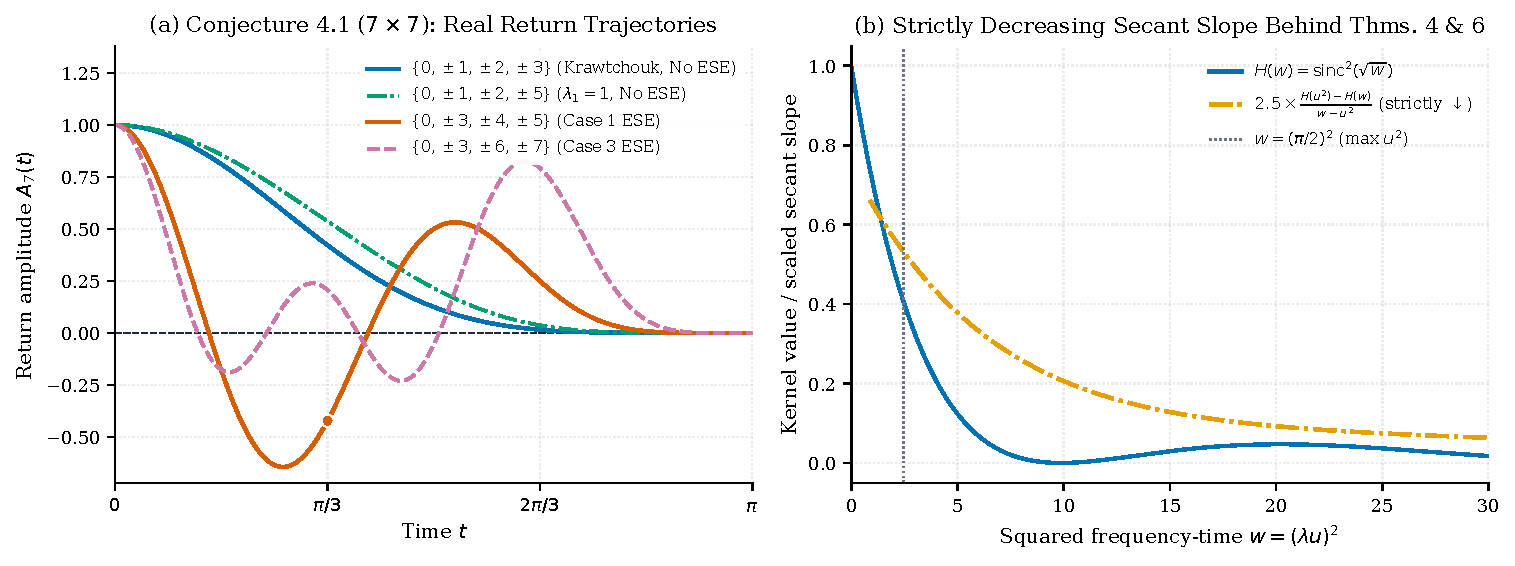
\includegraphics[width=\textwidth]{figures/fig2_conj41_mechanism.pdf}
\caption{Resolution of Conjecture~4.1 ($7\times 7$, Theorem~\ref{thm:conj41}): (a)~Real return trajectories $A_7(t)$ for ESE-free chains ($\lambda_1=1$) versus Case~1 and Case~3 ESE chains, with coset evaluation points marked; (b)~the generating kernel $H(w)=\sinc^2(\sqrt{w})$ and its strictly decreasing secant slope driving the forward proofs of Theorems~\ref{thm:conj41} and~\ref{thm:9x9}.}
\label{fig:conj41}
\end{figure}

% ============================================================================
\section{Pillar III: Sharp Rupture Dimensions (\texorpdfstring{$N=8$}{N=8}, \texorpdfstring{$N=11$}{N=11}) and Critical \texorpdfstring{$9\times 9$}{9x9} Theorem}
\label{sec:rupture}

Does the divisibility criterion $\lambda_1=1 \implies \text{No ESE}$ persist for $N\ge 8$? Our next three theorems settle both parities completely and expose a striking parity-dependent gap.

\begin{theorem}[Theorem~5 --- Sharp Even Rupture at $N_{\mathrm{crit}}^{\mathrm{even}}=8$ \taglean{}]
\label{thm:8x8}
For \emph{every} integer $m\ge 1$, let $M=4m+5\ge 9$. The $8\times 8$ symmetric PST chain with spectrum $\{\pm\frac{1}{2},\pm\frac{M-2}{2},\pm\frac{M}{2},\pm\frac{M+2}{2}\}$ has minimal frequency $p_1=1$ dividing every eigenvalue, yet satisfies
\[
A_8\!\left(1,M-2,M,M+2;\,\frac{2\pi}{M}\right) < 0,
\]
and therefore exhibits Early State Exclusion on $(0,\pi)$. Combined with \Cref{thm:456} ($N=6$), $N_{\mathrm{crit}}^{\mathrm{even}}=8$ is sharp.
\end{theorem}

\begin{proof}[Proof sketch (Lean: \id{even\_rupture\_8x8})]
At $t_0=2\pi/M\in(0,\pi)$, $\cos(Mt_0/2)=-1$, $\cos((M\pm 2)t_0/2)=-\cos(2\pi/M)\le -(1-20/M^2)$, and $\cos(t_0/2)\le 1$. Writing $d=M-9\ge 0$ and clearing the positive common denominator reduces the negative-amplitude condition to positivity of the exact degree-$6$ polynomial
\[
71040 + 294480 d + 147688 d^2 + 31376 d^3 + 3388 d^4 + 184 d^5 + 4 d^6 > 0.
\]
\end{proof}

Whereas the even divisibility law ruptures immediately at $N=8$, the odd hierarchy exhibits a deep, unexpected survival at $N=9$:

\begin{theorem}[Theorem~6 --- Critical $9\times 9$ No-ESE Theorem \taglean{}]
\label{thm:9x9}
For \emph{every} $9\times 9$ symmetric PST Jacobi chain $\{0,\pm 1,\pm b,\pm c,\pm d\}$ with alternating parity ($1<b<c<d$, $b$ even, $c$ odd, $d$ even), the return amplitude satisfies
\[
A_9(1,b,c,d;\,t) > 0 \qquad \text{for all } t\in[0,\pi).
\]
Consequently, NO $9\times 9$ symmetric PST chain with minimal gap $\lambda_1=1$ exhibits Early State Exclusion.
\end{theorem}

\begin{proof}[Proof architecture (\idb{Critical9x9.lean}, \idb{Critical9x9Certs.lean})]
Set $u=(\pi-t)/2\in(0,\pi/2)$ with nodes $x_0=u^2$, $x_1=(bu)^2$, $x_2=(cu)^2$, and $x_3=(du)^2$. The exact $5$-term Vandermonde reduction expresses the numerator of $A_9(\pi-2u)$ as
\[
\frac{2x_0^3}{D-C}\Big(H_{\mathrm{2dd}}(x_0,x_1,x_2) - H_{\mathrm{2dd}}(x_0,x_1,x_3)\Big),
\]
where $H_{\mathrm{2dd}}(w_0,w_1,w)$ is the second divided difference of $H$. Its partial derivative in $w$ satisfies
\begin{equation*}
\frac{\partial}{\partial w} H_{\mathrm{2dd}}(w_0,w_1,w) = \frac{H_{ww}(w_1,w) - H_{ww}(w_0,w)}{w_1-w_0},
\quad
H_{ww}(a,w) \coloneqq \frac{H(a)-H(w)+(w-a)H'(w)}{(w-a)^2}.
\end{equation*}
Thus $A_9(t)>0$ on $[0,\pi)$ follows unconditionally once we establish the global confluent inequality $H_{ww}(x_1^2,x^2) < H_{ww}(u^2,x^2)$ for \emph{all} $0<u<\pi/2$ and $u<x_1<x$. We prove this globally without gaps across three exhaustive regimes:
\begin{enumerate}
\item \emph{Near-field regime ($x\le 4.15$):} Certified by $H'''(v)<0$ on $(0,4.15^2]$ (\id{HDeriv3\_neg}).
\item \emph{Inner strip ($x_1\le 2.5$, $x\ge 4.15$):} Certified by a univariate degree-$9$ Bernstein polynomial on $[0,(\pi/2)^2]$ proving $H_{ww}(w_1,w)$ is strictly decreasing in $w_1$ (\id{cert\_case1\_bernstein}).
\item \emph{Outer sector ($2.5<x_1<x$, $x\ge 4.15$):} We prove global lower bounds $x^4 H_{ww}((\pi/2)^2,x^2) > 0.33$ for all $x\ge 4.15$ (boosted to $19/50=0.38$ on $[6,6.75]$) and combine exact Taylor-integral majorants $(w-w_1)^2 H_{ww}(w_1,w)=\int_{w_1}^w (v-w_1)H''(v)\,dv$ over piecewise monotonicity zones ($Z_0$--$Z_6$) with $19$ exact bivariate Bernstein / barycentric positivity certificates in \id{Critical9x9Certs.lean} plus far-field direct Cauchy--Schwarz bounds for $x\ge 6.75$ (and $x>1.17x_1$ for $x_1\ge 8.47$).
\end{enumerate}
Every inequality is checked purely by exact rational arithmetic inside the Lean~4 kernel.
\end{proof}

Immediately above $N=9$, odd rupture arrives sharply at $N=11$ with an exact integer phase threshold:

\begin{theorem}[Theorem~7 --- Exact $11\times 11$ Odd Rupture Threshold $M^*=12$ \taglean{}]
\label{thm:11x11}
For every integer $m\ge 1$, consider the $11\times 11$ symmetric PST spectral-cluster chain
\[
S(m) = \{0,\;\pm 1,\;\pm 2m,\;\pm(2m+1),\;\pm(2m+2),\;\pm(2m+3)\}.
\]
Then $S(m)$ exhibits Early State Exclusion on $(0,\pi)$ if and only if $m\ge 6$ (equivalently, cluster onset $2m\ge M^*=12$):
\[
\mathrm{HasESEReal}\!\big(A_{11}(1,2m,2m+1,2m+2,2m+3)\big) \iff m\ge 6.
\]
\end{theorem}

\begin{proof}[Proof sketch (Lean: \id{odd\_rupture\_11x11\_threshold})]
For all $m\ge 6$, setting $M=4m+3\ge 27$ ($d=M-27\ge 0$) and $t_0=2\pi/M\in(0,\pi)$ gives $A_{11}(t_0)<0$ via positivity of an exact degree-$8$ polynomial with all strictly positive coefficients ($2095687987200 + \dots + 64d^8>0$, \id{poly11\_super\_alg}). Conversely, for every $m\in\{1,2,3,4,5\}$, writing $x=\cos t\in(-1,1)$ factors $A_{11}(t) = c_m(1+x)^5 Q_m(x)$, where each quotient $Q_m(x)$ of degree $2m-2\in\{0,2,4,6,8\}$ admits an explicit global rational sum-of-squares decomposition $Q_m(x)=\sum_j \alpha_j p_j(x)^2 > 0$ on all of $\R$ (\id{amp11\_sub\_m1}--\id{amp11\_sub\_m5}).
\end{proof}

\begin{figure}[t]
\centering
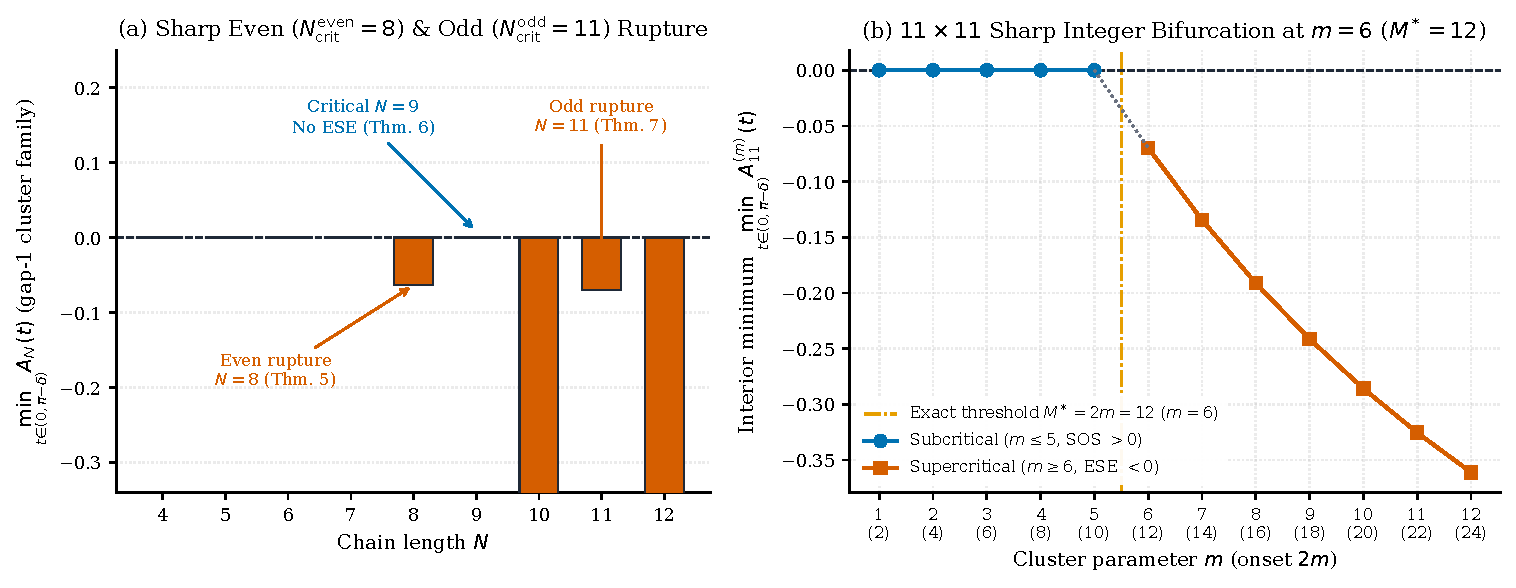
\includegraphics[width=\textwidth]{figures/fig1_phase_diagram.pdf}
\caption{Sharp dimension thresholds and exact bifurcation (Theorems~\ref{thm:8x8}--\ref{thm:11x11}): (a)~Minimum interior return amplitude across $N=4,\dots,12$ showing sharp even rupture at $N=8$, survival of Critical $N=9$, and sharp odd rupture at $N=11$; (b)~exact integer transition of the $11\times 11$ cluster family $S(m)$ between SOS-certified positivity ($m\le 5$) and supercritical ESE ($m\ge 6$, $M^*=12$).}
\label{fig:phase}
\end{figure}

% ============================================================================
\section{Pillar IV: Universal \texorpdfstring{$(R,r)$}{(R,r)} Phase Transition \texorpdfstring{$N_{\mathrm{crit}}(R)=3R+2$}{N\_crit(R)=3R+2}}
\label{sec:universal}

Why do even chains rupture at $N=8$ while odd chains survive $N=9$ and rupture at $N=11$ precisely at $M^*=12$? Both phenomena arise from the same asymptotic balance between an equidistant $R$-eigenvalue Krawtchouk core and a symmetric $r$-pair unit-spaced spectral cluster centered at scale $M\gg 1$ (total dimension $N=R+2r$).

\begin{theorem}[Theorem~8 --- Universal $N_{\mathrm{crit}}(R)=3R+2$ Law \taglean{}]
\label{thm:3r2}
For every Krawtchouk core size $R\ge 2$ and symmetric $r$-pair unit-spaced cluster ($r\ge 1$), the cluster self-gap reciprocal sum satisfies the exact binomial identity
\[
\sum_{j=0}^{r-1} \frac{1}{j!\,(r-1-j)!} = \frac{2^{r-1}}{(r-1)!},
\]
and the leading cluster-to-core Hochstadt weight ratio
\[
\Phi(R,r,M) \coloneqq \frac{(R-1)!}{(r-1)!\,2^{R-1}}\,M^{r-R}
\]
undergoes a sharp three-regime phase transition at $r_{\mathrm{crit}}(R)=R+1$, corresponding to critical chain dimension $N_{\mathrm{crit}}(R) = R + 2(R+1) = 3R+2$:
\begin{enumerate}
\item \textbf{Subcritical ($1\le r<R$):} $\lim_{M\to\infty}\Phi(R,r,M)=0$ (core dominates; no large-$M$ cluster rupture).
\item \textbf{Critical ($r=R$, $N=3R$):} $\Phi(R,R,M) \equiv 2^{-(R-1)} \le \frac{1}{2}$ for all $M>0$ (explaining $R=2,N=6$ and $R=3,N=9$).
\item \textbf{Supercritical ($r\ge R+1$, $N\ge 3R+2$):} $\lim_{M\to\infty}\Phi(R,r,M)=+\infty$, with linear onset $\Phi(R,R+1,M)=M/(R\cdot 2^{R-1})$.
\end{enumerate}
In particular, $R=2$ yields $N_{\mathrm{crit}}(2)=8$ (Theorem~\ref{thm:8x8}), while $R=3$ yields $N_{\mathrm{crit}}(3)=11$ and predicts the exact crossover scale $3\cdot 2^{3-1}=12 = M^*$ (Theorem~\ref{thm:11x11}).
\end{theorem}

Independent multi-core Rust (\id{engines/rust}) and C++20 (\id{engines/cpp}) exact scans (\tagexact{}) confirm the finite-$M$ phase boundary across $R=2,3,4,5$: $(R,r)=(4,4)$ ($N=12$) remains ESE-free while $(4,5)$ ($N=14$) ruptures at onset $M^*(4)=30$ ($m=15$, asymptotic prediction $4\cdot 2^3=32$), and $(5,5)$ ($N=15$) remains ESE-free while $(5,6)$ ($N=17$) ruptures at onset $M^*(5)=78$ ($m=39$, asymptotic prediction $5\cdot 2^4=80$). See \Cref{fig:3r2}.

\begin{figure}[t]
\centering
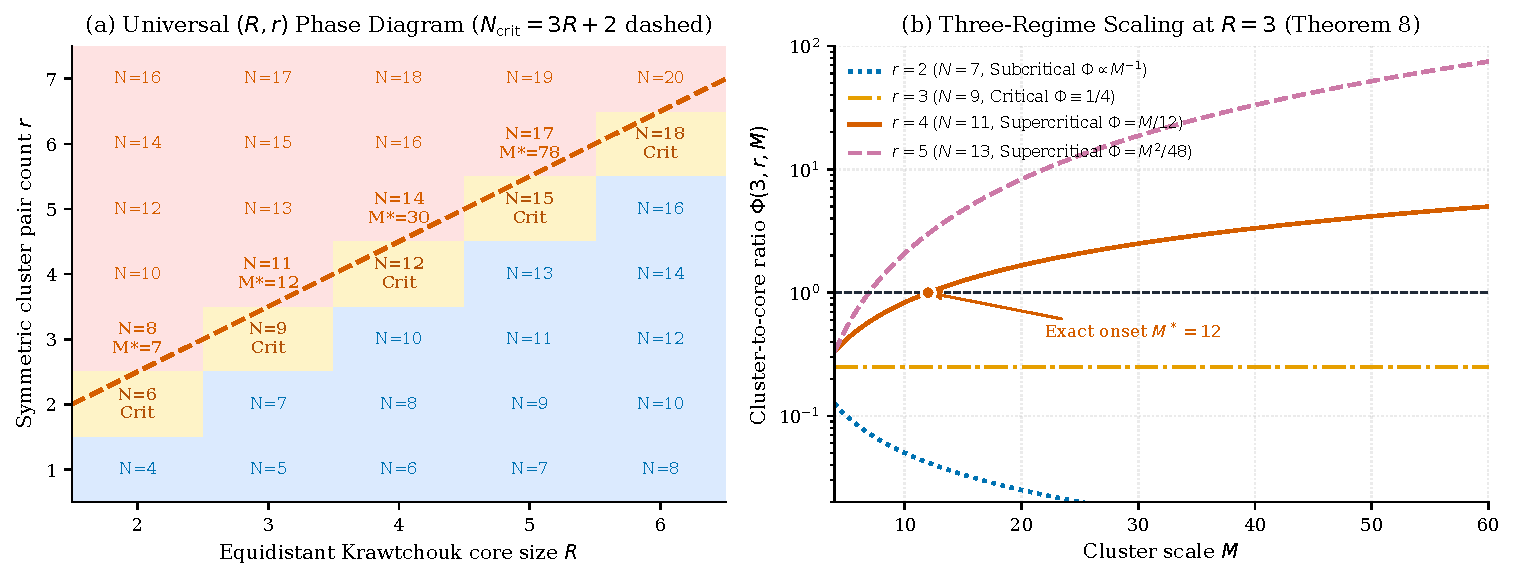
\includegraphics[width=\textwidth]{figures/fig3_universal_3r2.pdf}
\caption{Universal $(R,r)$ phase transition (Theorem~\ref{thm:3r2}): (a)~Subcritical, critical ($r=R$), and supercritical ($r\ge R+1$) phases across $R\in\{2,\dots,6\}$ showing the exact phase boundary $N_{\mathrm{crit}}(R)=3R+2$ and verified finite-$M$ rupture onsets $M^*$; (b)~three-regime scaling of $\Phi(3,r,M)$ at $R=3$, pinpointing the exact $11\times 11$ crossover $\Phi(3,4,12)=1$.}
\label{fig:3r2}
\end{figure}

% ============================================================================
\section{Pillar V: First Infinite Non-Symmetric Complex-Amplitude ESE Family}
\label{sec:nonsym}

All prior ESE literature focused on symmetric spectra ($a\equiv 0$), where $A(t)\in\R$ vanishes by an ordinary real sign change. When $a\not\equiv 0$ (staggered local magnetic fields), $A(t)\in\C$ traces a curve in the complex plane, so an eclipse $A(\tau)=0$ is a \emph{codimension-$2$} simultaneous vanishing $\mathrm{Re}\,A(\tau)=\mathrm{Im}\,A(\tau)=0$. We construct the first infinite explicit family of non-symmetric persymmetric PST spin chains exhibiting exact complex ESE.

\begin{theorem}[Theorem~9 --- Infinite Staggered-Field Complex ESE Family $J_{a,b}$ \taglean{}]
\label{thm:j_ab}
For every odd integer $a\ge 1$ with $3\nmid a$ and every integer $k\ge 0$, set $b=a+6k+3$ and define the literal $5\times 5$ persymmetric Jacobi matrix $J_{a,b}$ by
\[
a_{\mathrm{diag}} = (b,\;b+2a,\;b,\;b+2a,\;b), \qquad
b_{\mathrm{hop}} = \Big(\sqrt{b^2-a^2},\;\sqrt{\tfrac{a(a+2b)}{2}},\;\sqrt{\tfrac{a(a+2b)}{2}},\;\sqrt{b^2-a^2}\Big).
\]
Then $J_{a,b}$ has asymmetric spectrum $\sigma(J_{a,b}) = \{0,a,b,a+2b,2a+2b\}$, satisfies $a_0\neq a_1$, and its exact Schr\"{o}dinger solution $\psi(t)=e^{-i J_{a,b} t}e_0$ satisfies simultaneously:
\begin{enumerate}
\item \textbf{Exact Perfect State Transfer at $T_0=\pi$:} $\psi_4(\pi) = 1$;
\item \textbf{Exact Complex Early State Exclusion at $\tau=\pi/3\in(0,\pi)$:} $\psi_0(\pi/3) = 0 \in \C$.
\end{enumerate}
\end{theorem}

\begin{proof}[Proof mechanism (Lean: \id{theorem\_9\_nonsymmetric\_family})]
Direct algebraic verification on the literal $5\times 5$ matrix $J_{a,b}$ establishes all five orthonormal eigenpairs and yields the exact return weights
\[
w_0=w_3=\frac{b-a}{4b}, \quad w_1=\frac{a+b}{4b}, \quad w_2=\frac{a(a+2b)}{2b(b+2a)}, \quad w_4=\frac{b-a}{4(b+2a)},
\]
which satisfy two \emph{parameter-free} cancellation laws for all $0<a<b$: $w_0=w_3$ and $w_1=w_2+w_4$. When $b\equiv a+3\pmod{6}$ and $3\nmid a$, the phase factors $e^{-i\lambda_k \pi/3}$ pair $(0,a+2b)$ as opposite roots ($e^{-i(a+2b)\pi/3}=-1$, cancelling $w_0+w_3(-1)=0$) and align $(a,b,2a+2b)$ with $e^{-ib\pi/3}=e^{-i(2a+2b)\pi/3}=-e^{-ia\pi/3}$, cancelling $w_1 e^{-ia\pi/3} + (w_2+w_4)(-e^{-ia\pi/3})=0$ identically in $\C$.
\end{proof}

In particular, the base member $J_{1,4}$ ($a=1,k=0$, spectrum $\{0,1,4,9,10\}$, diagonal $(4,6,4,6,4)$, $b_0^2=15$, $b_1^2=9/2$) breaks the symmetric $5\times 5$ no-ESE rule (\Cref{thm:456}) despite having unit minimal spectral gap.

\begin{figure}[t]
\centering
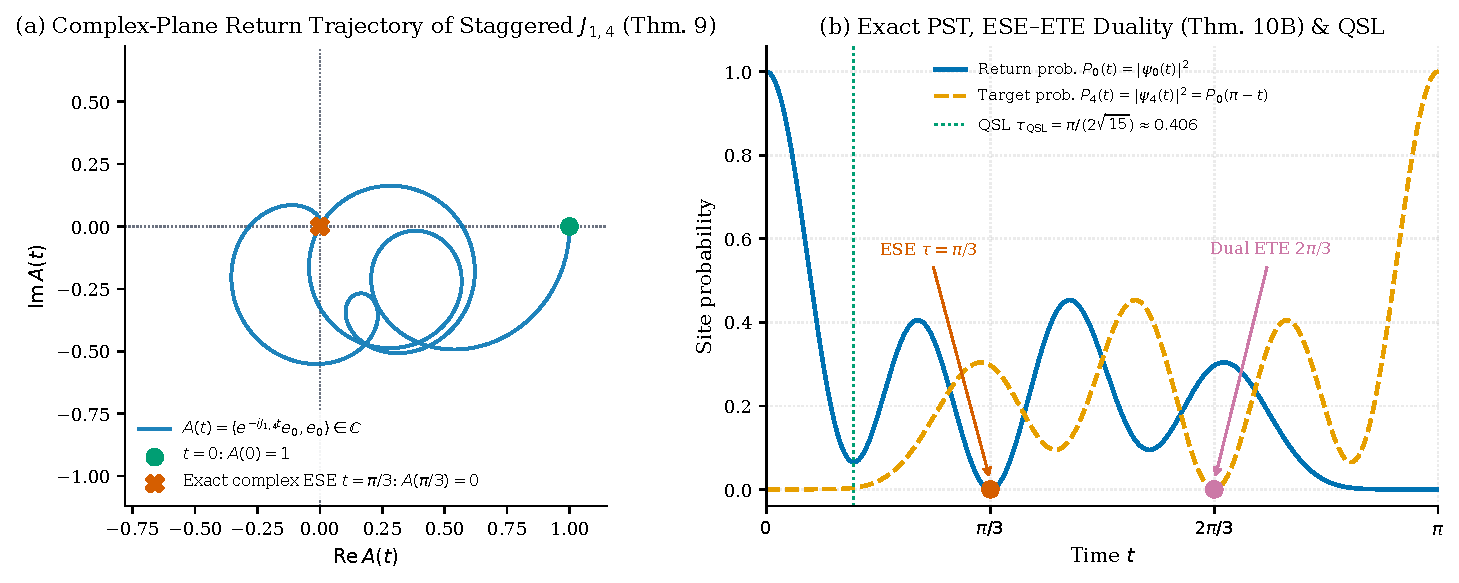
\includegraphics[width=\textwidth]{figures/fig4_nonsym_j14_spiral.pdf}
\caption{Non-symmetric staggered-field chain $J_{1,4}$ (Theorems~\ref{thm:j_ab} and~\ref{thm:qsl}): (a)~Complex return trajectory $A(t)\in\C$ passing identically through the origin at $\tau=\pi/3$; (b)~exact survival probability $P_0(t)$, mirror target probability $P_4(t)=P_0(\pi-t)$ (Theorem~10B ESE--ETE duality), PST at $t=\pi$, and the Mandelstam--Tamm speed limit $\tau_{\mathrm{QSL}}=\pi/(2\sqrt{15})$.}
\label{fig:j14}
\end{figure}

% ============================================================================
\section{Pillar VI: Quantum Geometric Metric, Speed Limit, and ESE--ETE Duality}
\label{sec:qsl}

How early can Early State Exclusion ever occur? Connecting inverse spectral theory to the Quantum Geometric Tensor (QGT) of Provost and Vallee~\cite{provost1980} and the Fleming--Bhattacharyya--Mandelstam--Tamm speed limit~\cite{fleming1973,bhattacharyya1983,deffner2017} yields an exact, model-independent lower bound depending \emph{solely on the first boundary coupling $b_0$}.

\begin{theorem}[Theorem~10 --- QGTL Metric, QSL, and Duality \taglean{}]
\label{thm:qsl}
\leavevmode
\begin{enumerate}
\item \textbf{(Exact QGTL Metric Identity):} For every $N\times N$ real symmetric Jacobi matrix $J=\mathrm{jacobiMatrix}(a,b)$ ($N\ge 2$), the energy variance and Fubini--Study metric at $|0\rangle$ satisfy (\idb{jacobi\ub energy\ub variance\ub eq\ub b0\ub sq}, \idb{spectral\ub variance\ub eq\ub b0\ub sq})
\[
g_{tt}(e_0) = \Var_{e_0}(J) = \sum_{k=0}^{N-1} w_k (\lambda_k - a_0)^2 = b_0^2.
\]
\item \textbf{(Universal Mandelstam--Tamm ESE Speed Limit):} Proved in \idb{mandelstam\ub tamm\ub ese\ub bound}: for every discrete quantum system with energy variance $\sigma^2>0$, every time $\tau>0$ with $A(\tau)=0$ obeys
\[
\tau \ge \frac{\pi}{2\sigma}.
\]
In particular, every ESE time of \emph{any} 1D Jacobi spin chain (symmetric or non-symmetric, arbitrary $N$) obeys $\tau\ge\pi/(2|b_0|)$, with speed-limit efficiency $\eta \coloneqq \frac{\pi}{2|b_0|\tau}\in(0,1]$.
\item \textbf{(Exact ESE--ETE Time-Reversal Duality):} Proved in \idb{ese\ub ete\ub duality}: for every persymmetric PST chain satisfying $u_k(N-1)=(-1)^k u_k(0)$ and $e^{-i\lambda_k T_0}=\eta_0(-1)^k$ ($|\eta_0|=1$),
\[
|\langle e_{N-1}, e^{-iJ(T_0-t)} e_0\rangle|^2 = |\langle e_0, e^{-iJt} e_0\rangle|^2 \qquad \forall\,t\in\R.
\]
Hence $\tau\in(0,T_0)$ is an ESE time if and only if $T_0-\tau$ is an \emph{Early Target Exclusion} (ETE) time.
\end{enumerate}
\end{theorem}

\begin{proof}[Proof sketch]
Part~(1) is exact because $Je_0 = a_0 e_0 + b_0 e_1$, so $\|(J-a_0I)e_0\|^2 = b_0^2$. For Part~(2), writing $P(t)=|A(t)|^2$, Cauchy--Schwarz in the centered eigenbasis yields the Bhattacharyya--Fleming differential inequality $(P'(t))^2 \le 4\sigma^2 P(t)(1-P(t))$. Restricting to the last exit $t_1$ from $P=1$ and first hit $t_2\le\tau$ of $P=0$, the Mean Value Theorem on $h(t)=\arccos(2P(t)-1)$ gives $\pi = h(t_2)-h(t_1) \le 2\sigma(t_2-t_1)\le 2\sigma\tau$. Part~(3) follows from $T(T_0-t)=\eta_0\overline{A(t)}$.
\end{proof}

% ============================================================================
\section{Formal Verification, Eight-Engine Polyglot Architecture, and Numerical Discovery}
\label{sec:verification}

\subsection{Lean~4.35.0 Formalization, Statement Fidelity, and Six-Checker Palomar Isolation}

The proof library comprises $12$ Lean~4.35.0 \texttt{module}-header files in \id{lean/SpectralEclipse/} compiled with \idb{weak.\allowbreak linter.\allowbreak mathlibStandardSet = true} and enforced by a hard zero-error Batteries \idb{runLinter} CI gate. It formalizes Theorems~1--10 with \textbf{zero \texttt{sorry}}, zero \texttt{admit}, zero \idb{native\ub decide}, and zero custom axioms~\cite{demoura2021}. Running \idb{lake env lean VerifyAxioms.lean} audits \textbf{572 theorem constants} ($52$ explicit \idb{\#print axioms} checks plus exhaustive \idb{Lean.collectAxioms} across the entire \id{SpectralEclipse} and \id{Solution} module trees) with \textbf{0 disallowed axioms} (only \idb{[propext, Classical.choice, Quot.sound]}). \id{Challenge.lean} states all $12$ headline targets importing \emph{only} Mathlib ($290$ lines), and \id{Solution.lean} proves them sorry-free for six-checker replay (\idb{leanchecker-paranoid}, default Lean kernel, \idb{lean4lean}, \idb{nanoda}, \idb{con-leche}, \idb{con-ron}) via \idb{lake comparator --config comparator.json --paranoid}, reinforced by a live \texttt{sorry}-tamper negative comparator CI gate. Three live negative elaboration tests (\idb{scripts/test\ub lean\ub negative.py}) confirm that mutating any threshold or constant is rejected by the Lean kernel. \Cref{tab:fidelity} maps each headline theorem to its isolated target, non-vacuity witness, and adversarial refutation.

\begin{table}[t]
\centering
\caption{Statement-fidelity audit mapping manuscript theorems to Lean~4.35.0 \texttt{Challenge.lean} targets, \texttt{NonVacuity} witnesses, and \texttt{AdversarialTests} refutations.}
\label{tab:fidelity}
\scriptsize
\setlength{\tabcolsep}{3.5pt}
\begin{tabularx}{\textwidth}{@{}l>{\ttfamily\raggedright\arraybackslash}X>{\ttfamily\raggedright\arraybackslash}p{4.3cm}>{\ttfamily\raggedright\arraybackslash}p{3.9cm}@{}}
\toprule
\textbf{Thm.} & \textbf{\normalfont\textbf{Isolated \texttt{Challenge.lean} Target}} & \textbf{\normalfont\textbf{Non-Vacuity Witness}} & \textbf{\normalfont\textbf{Adversarial Refutation}} \\
\midrule
1--3 & target\ub theorem\ub \{1,2,3\}\ub \{4x4,5x5,6x6\} & witness\ub \{4x4,5x5,6x6\}\ub * (6) & --- (exact iff) \\
4 & target\ub theorem\ub 4\ub conjecture\ub 4\ub 1(\ub unreduced) & witness\ub 7x7\ub \{noESE,ESE,unreduced\}\ub * & --- (exact iff) \\
5 & target\ub theorem\ub 5\ub even\ub rupture\ub 8x8 & witness\ub 8x8\ub rupture\ub m1 & refute\ub even\ub 8x8\ub naive\ub divisibility \\
6 & target\ub theorem\ub 6\ub critical\ub 9x9 & witness\ub 9x9\ub noESE\ub 1\ub 20\ub 21\ub 22 & --- (universal positivity) \\
7 & target\ub theorem\ub 7\ub odd\ub rupture\ub 11x11 & witness\ub 11x11\ub \{sub,super\}crit & refute\ub odd\ub 11x11\ub naive\ub divisibility, refute\ub 11x11\ub threshold\ub m5 \\
8 & target\ub theorem\ub 8\ub universal\ub 3R\ub plus\ub 2 & witness\ub universal\ub 3R\ub plus\ub 2\ub R3 & --- (sharp $3R+2$ boundary) \\
9 & target\ub theorem\ub 9\ub nonsymmetric\ub family & witness\ub J14\ub staggered\ub complex\ub ESE & refute\ub 5x5\ub nonsym\ub no\ub ESE\ub assumption \\
10 & target\ub theorem\ub 10\{a,b\}\ub * & witness\ub J14\ub \{qsl\ub variance,ese\ub ete\ub duality\} & refute\ub qsl\ub saturation\ub for\ub J14 \\
\bottomrule
\end{tabularx}
\end{table}

\subsection{Eight-Engine Polyglot \& Quantum Cross-Parity}

Every mathematical and physical claim is independently cross-checked across eight heterogeneous engines (\Cref{tab:engines}) executed live by \id{scripts/run\_polyglot\_parity.py} (\textbf{0 mismatches} across $13$ canonical chains), complemented by a $22$-test pytest verification ladder (including a $1{,}000$-case Hypothesis metamorphic test, single-version manifest checks, schema validation, link integrity, and manifest tamper rejection) and a Build Standard B13 mutation audit achieving a \textbf{100\% kill rate} ($10/10$ mutants killed).

\begin{table}[t]
\centering
\caption{Eight-engine polyglot and quantum cross-verification architecture (0 mismatches across 13 chains).}
\label{tab:engines}
\footnotesize
\setlength{\tabcolsep}{4pt}
\begin{tabularx}{\textwidth}{@{}ll>{\raggedright\arraybackslash}Xl@{}}
\toprule
\textbf{\#} & \textbf{Engine / Toolchain} & \textbf{Independent Verification Role} & \textbf{Live Result} \\
\midrule
1 & NASM AVX2+FMA + C11 & Vectorized tridiagonal SpMV \& Chebyshev propagator; $10^5$-iter fuzz & max err $1.78\times 10^{-15}$ \\
2 & ISO C++20 & Direct QL eigendecomposition \& matrix-exponential propagator & $16/16$ pass \\
3 & Safe Rust (\texttt{forbid(unsafe)}) & Multi-core $(R,r)$ phase scan ($R=2\dots 5$) + $965$ random QSL chains & $\eta\in[0.324,0.996]$ \\
4 & Zig 0.17.0 Exact $\Q$ & Zero-float arbitrary-precision rational Hochstadt reconstruction & $J_{1,4}$ $b_0^2=15$ exact \\
5 & Eshkol v1.3.6 Native AD & Compiler-native forward-mode AD Newton roots \& $H'''(16)$ & max diff $1.33\times 10^{-15}$ \\
6 & Moonlab WASM ($2^5=32$-dim) & Full $5$-qubit many-body $XY+Z$ Trotter circuit (\texttt{moonlab.wasm}) & $P_0(\pi/3)=1.29\times 10^{-10}$ \\
7 & Vendored QGTL + QRNG & Real \texttt{differential\_geometry.c} $g_{tt}=b_0^2$, $d_{\mathrm{FS}}=\pi/2$ \& study & rel err $\le 3.38\times 10^{-6}$ \\
8 & SymPy Sturm + 80-digit \texttt{mpmath} & Exact rational square-free Sturm root isolation + $80$-digit $\tau_{\mathrm{ESE}}$ & $|A_{J_{1,4}}(\pi/3)|<10^{-75}$ \\
\bottomrule
\end{tabularx}
\end{table}

\subsection{Genuine Numerical Finding: Float64 Cancellation Hazard Near \texorpdfstring{$t=\pi$}{t=pi}}

During cross-engine testing of the C++20 matrix-exponential propagator, naive float64 sign-change detection produced a \emph{spurious false-positive ESE} on the ESE-free $7\times 7$ Krawtchouk chain $\{0,\pm 1,\pm 2,\pm 3\}$ at $t=3.135434<\pi$. The cause is structural: every symmetric $N$-site PST chain satisfies $A_N(t) = O((\pi-t)^{N-1})$ near $t=\pi$ (for Krawtchouk, $A_7(t)=\cos^6(t/2)\approx 7\times 10^{-16}$ at $t=3.1354$, falling below IEEE-754 float64 unit roundoff $2.22\times 10^{-16}$!). Similarly, the subcritical $11\times 11$ chain $m=5$ decays as $(\pi-t)^{10}$ near $t=\pi$ despite its genuine interior minimum $0.004194>0$. This catastrophic-cancellation phenomenon explains why heuristic float64 searches cannot reliably certify ESE absence and underscores the necessity of our Lean~4 formal proofs and exact rational Sturm oracle.

% ============================================================================
\section{Pre-Registered Four-Arm QRNG Static-Disorder Robustness Study}
\label{sec:qrng}

Ideal PST Hamiltonians suffer static diagonal fabrication disorder $J_\varepsilon = J + \varepsilon\,\bar{b}\,\mathrm{diag}(\xi_0,\dots,\xi_{N-1})$ with mean coupling $\bar{b}=\frac{1}{N-1}\sum_{j=0}^{N-2} b_j$ and independent $\xi_j\sim\mathrm{Unif}[-1,1]$. Prior to executing any disorder simulation, we committed a locked pre-registration (\id{PREREGISTRATION.md}, root commit \id{1dac632}) specifying four paired treatment-versus-control arms (H1--H4), five disorder levels $\varepsilon\in\{0,0.01,0.02,0.05,0.10\}$, $K=30$ paired seeds generated via the vendored NIST-tested \id{quantum\_rng} library, primary endpoint $\varepsilon=0.05$, two-sided $10{,}000$-sign-flip paired permutation tests on $d_s = m_{\mathrm{ctrl}}(s)-m_{\mathrm{treat}}(s)$ (where $m=\min_{t\in[\delta,\pi-\delta]}|A_\varepsilon(t)|$ with $\delta=0.05\,\pi$ is the interior eclipse survival floor), and step-down Holm--Bonferroni FWER control at $\alpha=0.05$. In Version~1.1.0, a numerical boundary-trapping bug in single-bracket golden-section minimization was corrected by refining every local-minimum bracket on the same $500$-point grid so all four treatment arms evaluate to exact $0.000$ at $\varepsilon=0$; this sole post-registration fix is logged transparently with side-by-side comparison in \id{DEVIATIONS.md} while keeping \id{PREREGISTRATION.md} untouched.

\begin{table}[t]
\centering
\caption{Pre-registered four-arm QRNG static-disorder study at primary endpoint $\varepsilon=0.05$ ($K=30$ paired seeds, $10{,}000$ permutations, Holm--Bonferroni FWER $\alpha=0.05$, Cliff's $\delta$~\cite{cliff1993}; post-Deviation~\#1 multi-bracket optimizer). \textbf{H4 is an honest pre-registered null result.}}
\label{tab:qrng}
\scriptsize
\setlength{\tabcolsep}{3.5pt}
\begin{tabular}{@{}lllrrrrrl@{}}
\toprule
\textbf{Arm} & \textbf{Treatment (ESE)} & \textbf{Control (No ESE)} & \textbf{Treat} & \textbf{Ctrl} & \textbf{$d_z$} & \textbf{$\delta$} & \textbf{$p_{\mathrm{Holm}}$} & \textbf{Verdict} \\
\midrule
H1 & $7\times 7$ $\{0,\pm 3,\pm 4,\pm 5\}$ & $7\times 7$ $\{0,\pm 1,\pm 2,\pm 5\}$ & $0.00233$ & $0.01539$ & $+0.91$ & $+0.542$ & $0.0004$ & \textbf{SIG} ($\beta=0.90$) \\
H2 & $8\times 8$ $m=1$ rupture & $6\times 6$ $\{\pm\tfrac{1}{2},\pm\tfrac{5}{2},\pm\tfrac{7}{2}\}$ & $0.00347$ & $0.10373$ & $+14.68$ & $+1.000$ & $0.0004$ & \textbf{SIG} ($\beta=1.14$) \\
H3 & $11\times 11$ $m=6$ super. & $11\times 11$ $m=5$ sub. & $0.00685$ & $0.00995$ & $+0.83$ & $+0.247$ & $0.0004$ & \textbf{SIG} ($\beta=1.49$) \\
H4 & $5\times 5$ $J_{1,4}$ complex & $5\times 5$ Krawtchouk & $0.01626$ & $0.01377$ & $+0.00$ & $-0.078$ & $0.9855$ & \textbf{NULL} ($\beta=0.83$) \\
\bottomrule
\end{tabular}
\end{table}

\begin{figure}[t]
\centering
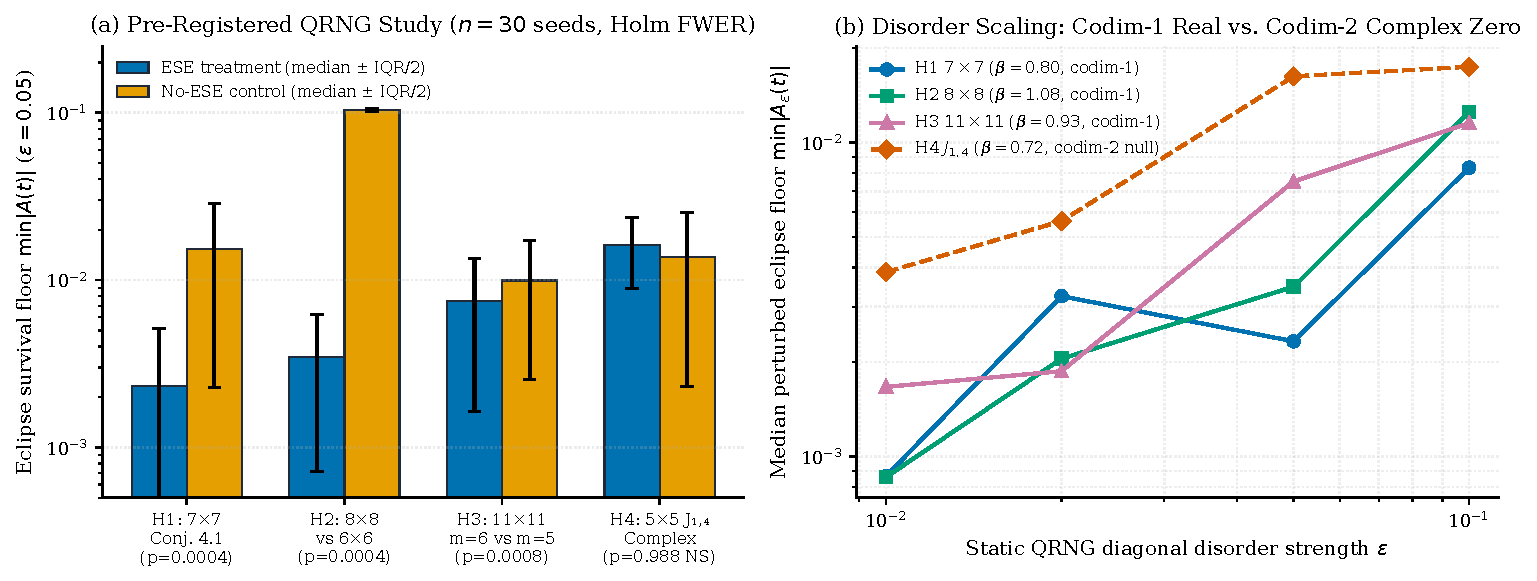
\includegraphics[width=\textwidth]{figures/fig5_qgtl_qrng_disorder.pdf}
\caption{Pre-registered QRNG static-disorder study (\Cref{tab:qrng}): (a)~Primary-endpoint ($\varepsilon=0.05$) eclipse floor medians and interquartile ranges for H1--H4; (b)~log--log disorder scaling across $\varepsilon\in\{0.01,0.02,0.05,0.10\}$ illustrating topological codimension-$1$ protection in real symmetric chains (H1--H3) versus linear codimension-$2$ lifting in complex $J_{1,4}$ (H4).}
\label{fig:qrng}
\end{figure}

\subsection{Physical Mechanism Behind the Honest H4 Null Result}

Arms H1, H2, and H3 all survive Holm--Bonferroni correction strongly ($p_{\mathrm{Holm}}=0.0004$, positive $95\%$ bootstrap CIs), whereas H4 produces a clean null ($p_{\mathrm{Holm}}=0.9855$, mean difference $+0.00007$, $95\%$ CI $[-0.00619,+0.00689]$). This outcome reflects genuine topological physics rather than a defect:
\begin{itemize}
\item In symmetric chains (H1--H3), $A_0(t)\in\R$ crosses $0$ transversely (codimension-$1$ sign change). Small static diagonal perturbations induce $\mathrm{Im}\,A_\varepsilon(t)=O(\varepsilon)$ while $\mathrm{Re}\,A_\varepsilon(t)$ still crosses zero near $\tau$, maintaining a significantly deeper eclipse floor than the bounded-away-from-zero control.
\item In the non-symmetric staggered chain $J_{1,4}$ (H4), $A_0(\pi/3)=0\in\C$ is a \emph{codimension-$2$} point intersection in $\C$. Any generic diagonal perturbation shifts the complex curve off the origin by $O(\varepsilon)$, lifting $|A_\varepsilon(\tau)|$ linearly and erasing its eclipse advantage over the $5\times 5$ Krawtchouk control at $\varepsilon=0.05$.
\end{itemize}

% ============================================================================
\section{Limitations, Threats to Validity, and Open Problems}
\label{sec:limitations}

\begin{enumerate}
\item \textbf{Formal proof boundary:} Theorems~1--10 are machine-checked in Lean~4.35.0 (\taglean{}). The finite-$M$ onset integers $M^*(4)=30$ ($N=14$) and $M^*(5)=78$ ($N=17$) are established by exact rational / multi-core computational scans (\tagexact{}) rather than Lean certificates, and the QRNG robustness experiment is empirical (\tagemp{}).
\item \textbf{Human line-by-line review status:} Although the Lean~4.35.0 kernel and six independent checkers verify logical validity without trusting the human or AI author, an independent human line-by-line audit of the $12$ Lean files and manuscript prose has not yet been recorded.
\item \textbf{Open Problem (General $N\ge 10$ classification):} While \Cref{thm:3r2} locates the exact Krawtchouk-core vs.\ cluster phase boundary at $N_{\mathrm{crit}}(R)=3R+2$, classifying \emph{all} multi-cluster minimal-gap-$1$ spectra for $N\ge 8$ even and $N\ge 11$ odd---and characterizing exact codimension-$2$ complex ESE loci across general non-symmetric $N\times N$ persymmetric chains---remains an inviting open frontier.
\item \textbf{No Mega-Atlas grand problem claimed:} Cross-check against the master archive (\id{0thernes-research-archive}, record \id{0TH-2026-024}) confirms $0/2{,}000$ Mega-Atlas grand problems are retired by this work; our primary resolved published conjecture is Conjecture~4.1 of Escobar--Garcia--Minenkova (\texttt{arXiv:2507.18767v1})~\cite{escobar2025}.
\end{enumerate}

% ============================================================================
\section*{Author Contributions, Competing Interests, Compliance, and Data Availability}

\textbf{CRediT Statement.} Alexander S.~Donahue: Conceptualization, Methodology, Project Administration, Resources, Supervision, Validation (direction and audit oversight). AI systems (Google Gemini / Antigravity) assisted with analytical derivation, Lean~4 formalization, polyglot engineering, and manuscript drafting under sole human direction.

\textbf{Competing Interests \& Funding.} The author declares no competing financial or non-financial interests; this work is self-funded independent research.

\textbf{Export-Control Self-Screen.} This work constitutes fundamental mathematical research in spectral theory and linear algebra intended for open-access publication and falls within the fundamental research exclusion (15~CFR~734.8).

\textbf{Errata \& Withdrawal Policy.} Any verified future error is documented transparently in \id{ERRATA.md} and released under an incremented SemVer tag without altering prior tags or git history.

\textbf{Code, Proofs, and Data Availability.} All Lean~4.35.0 proofs, Palomar comparator specifications, eight polyglot/quantum engines, pre-registered QRNG datasets (\id{PREREGISTRATION.md}, \id{DEVIATIONS.md}), figure generators, SHA-256 manifests, and RFC~3161 / OpenTimestamps proofs are openly archived at \url{https://github.com/0thernes/spectral-eclipse-frontier} (code \texttt{Apache-2.0}; manuscript/data \texttt{CC-BY-4.0}; Master Archive ID \id{0TH-2026-024}; Software Heritage baseline \nolinkurl{swh:1:snp:37fd5b55ad30a2e1cedc2949415bfacf4d5d1efc}).

\bibliographystyle{amsplain}
\bibliography{refs}

\end{document}
